\chapter{Final Result} \label{chap:6}

The final result based on the 95$\% $ CLs of upper limit on signal cross section $\times $ branch ratio (pp $\rightarrow$ X $\rightarrow$ HH $\rightarrow b\bar{b}b\bar{b}$) is shown in the chpter.

\section{Asymptotic CLs} 
The analysis uses CLs to find the upper limit of cross section\citep{0954-3899-28-10-313,NicolasChanon}. The CLs method tests whether the data is more consistent with a signal + background hypothesis or with a background-only hypothesis when the statistic of data is low. The CLs method starts with calculating likelood ration of the two hypotheses. 
\begin{equation} \label{eq1}
\begin{split}
Q = \frac{\textbf{\textsl{L}}(\textsl{N}_{data},\textsl{N}_{S}+\textsl{N}_{B})}{\textbf{\textsl{L}}(\textsl{N}_{data},\textsl{N}_{B})}\\
\textbf{\textsl{L}}(n,x) = \frac{e^{-x}}{n!}x^n
\end{split}
\end{equation}
Then, the prabability density function on -2$\textit{ln}$(Q) of the two hypotheses are generated by toy-experiments using $\textsl{N}_{S} + \textsl{N}+{B}$ and $\textsl{N}+{B}$ as $\textsl{N}_{data}$ in the equation separately. The $CL_{s+b}$ represents the prabability of results less consisentent with a signal + background hypothesis, while the $CL_{b}$ represents the prabability of results less consisentent with a background-only hypothesis.
\begin{equation} \label{eq1}
\begin{split}
CL_{s+b} = P_{s+b}(lnQ \leq lnQ_{obs}) = \int^{lnQ_{obs}}_{-\infty} \frac{dP_{s+b}}{dlnQ} dlnQ \\
CL_{b} = P_{b}(lnQ \leq lnQ_{obs}) = \int^{lnQ_{obs}}_{-\infty} \frac{dP_{b}}{dlnQ} dlnQ
\end{split}
\end{equation}
The CLs defined as 
\begin{equation} \label{eq1}
\begin{split}
CL_{s} = \frac{CL_{s+b}}{CL_{b}}
\end{split}
\end{equation}
can be approximately seen as signal-only hypothesis. The 95$\% $ confidence level of CLs means that the prabability to observed the data excessing the signal + background hypothesis which is normalized to the prabability to observed the data excessing the background-only hypothesis is less thna 5 $\% $. The observed  exclusion of 95$\% $ confidence level of CLs is calculated by integrated to a given $lnQ_{obs}$ where CLs $<$ 0.05. The expected exclusion limit is done in same procedure where $lnQ_{obs}$ is replaced by $lnQ_{b}$ in the equation. The Asymptotic CLs is obtained by CMS Higgs combination tool\citep{higgsCombine}.

\clearpage
\section{95$\% $ upper limit}
The figure 6.1 shows the 95$\% $ upper limit on signal cross section $\times $ branch ratio (pp $\rightarrow$ X $\rightarrow$ HH $\rightarrow b\bar{b}b\bar{b}$) of both signal. For bulk graviton, we didn't exclude any region, and the upper limit is below 10 fb with k/M$_{Pl}$ = 0.1. On the other hand, we excluded the region of m$_{R}$ below 1787 GeV and from   considering $\Lambda_{R}$ = #TeV.

 \begin{figure}[t]
  \centering
 \begin{tabular}{cc}
    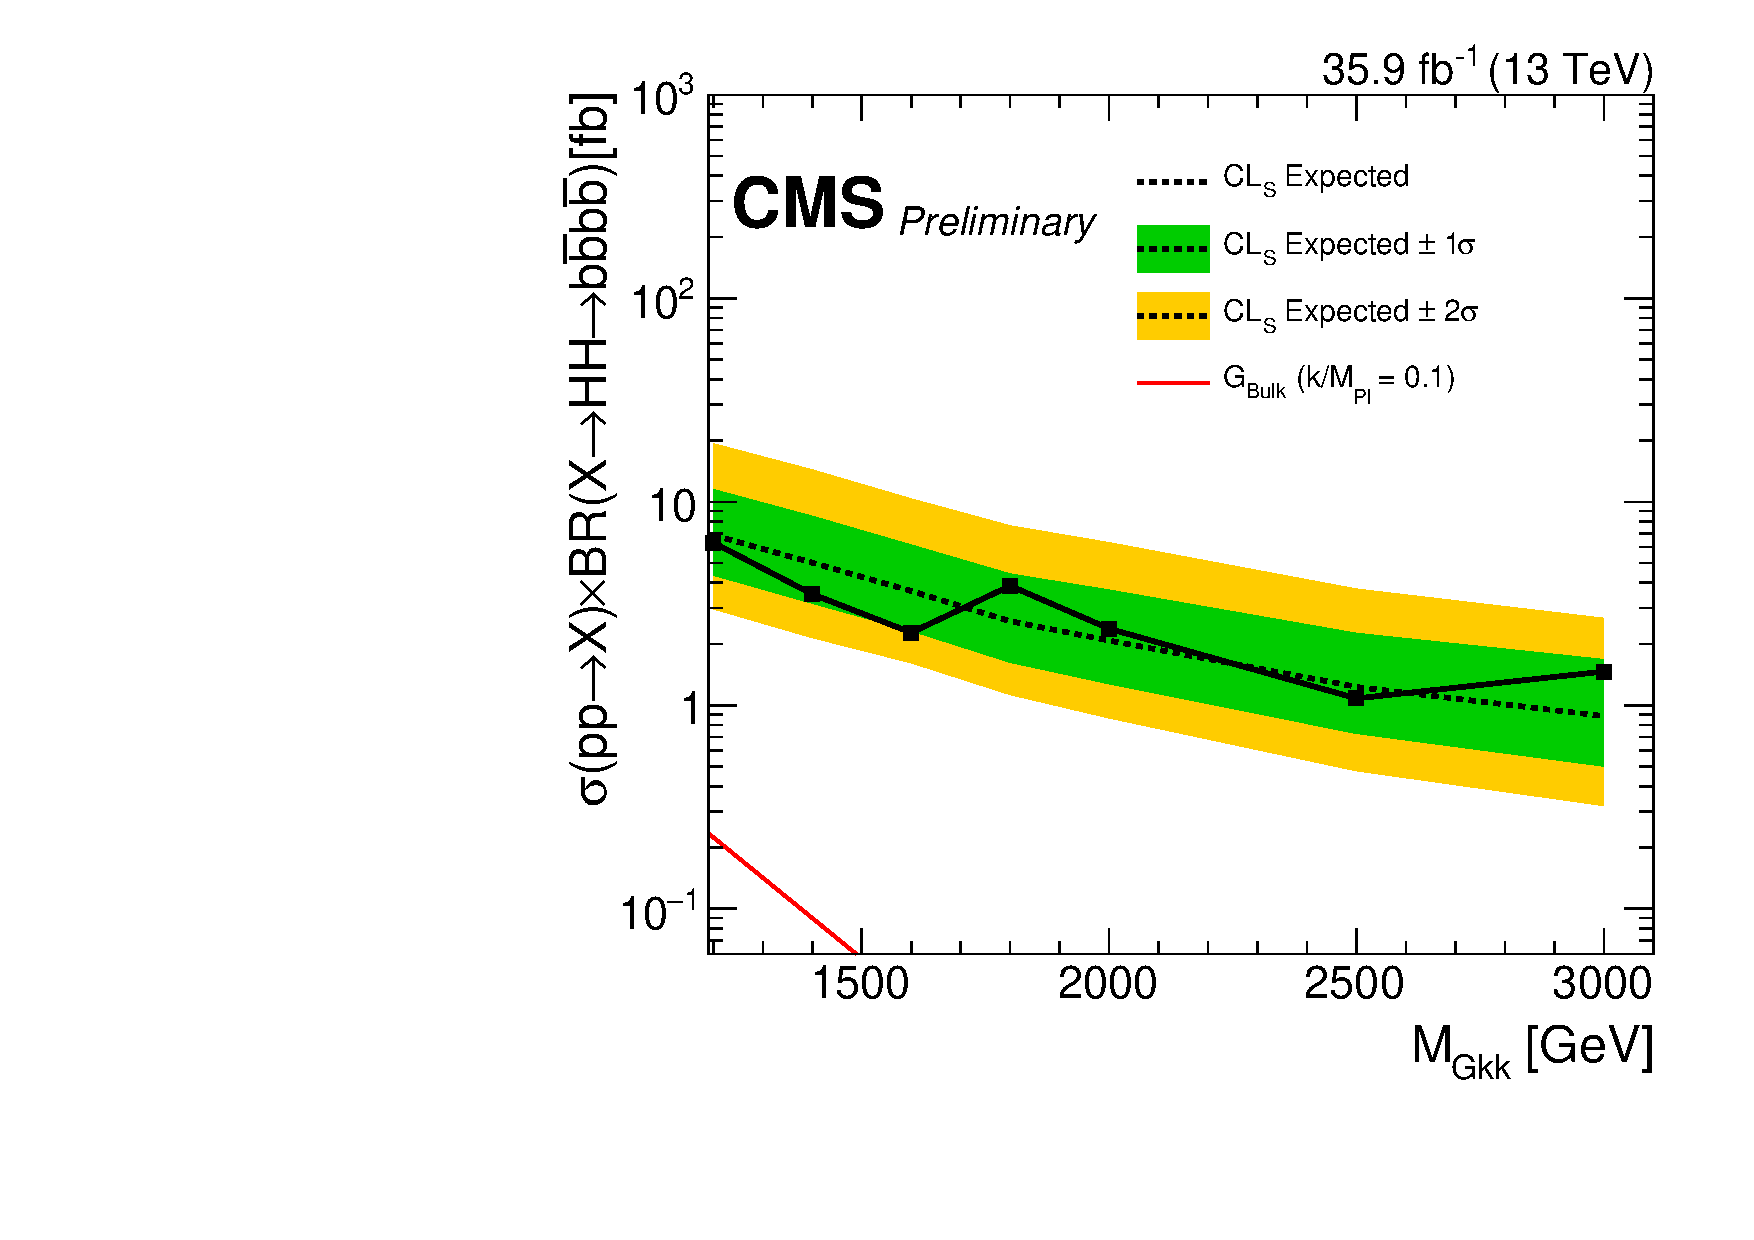
\includegraphics[width=0.5\textwidth]{Figures/central_CW/limit.pdf} &
   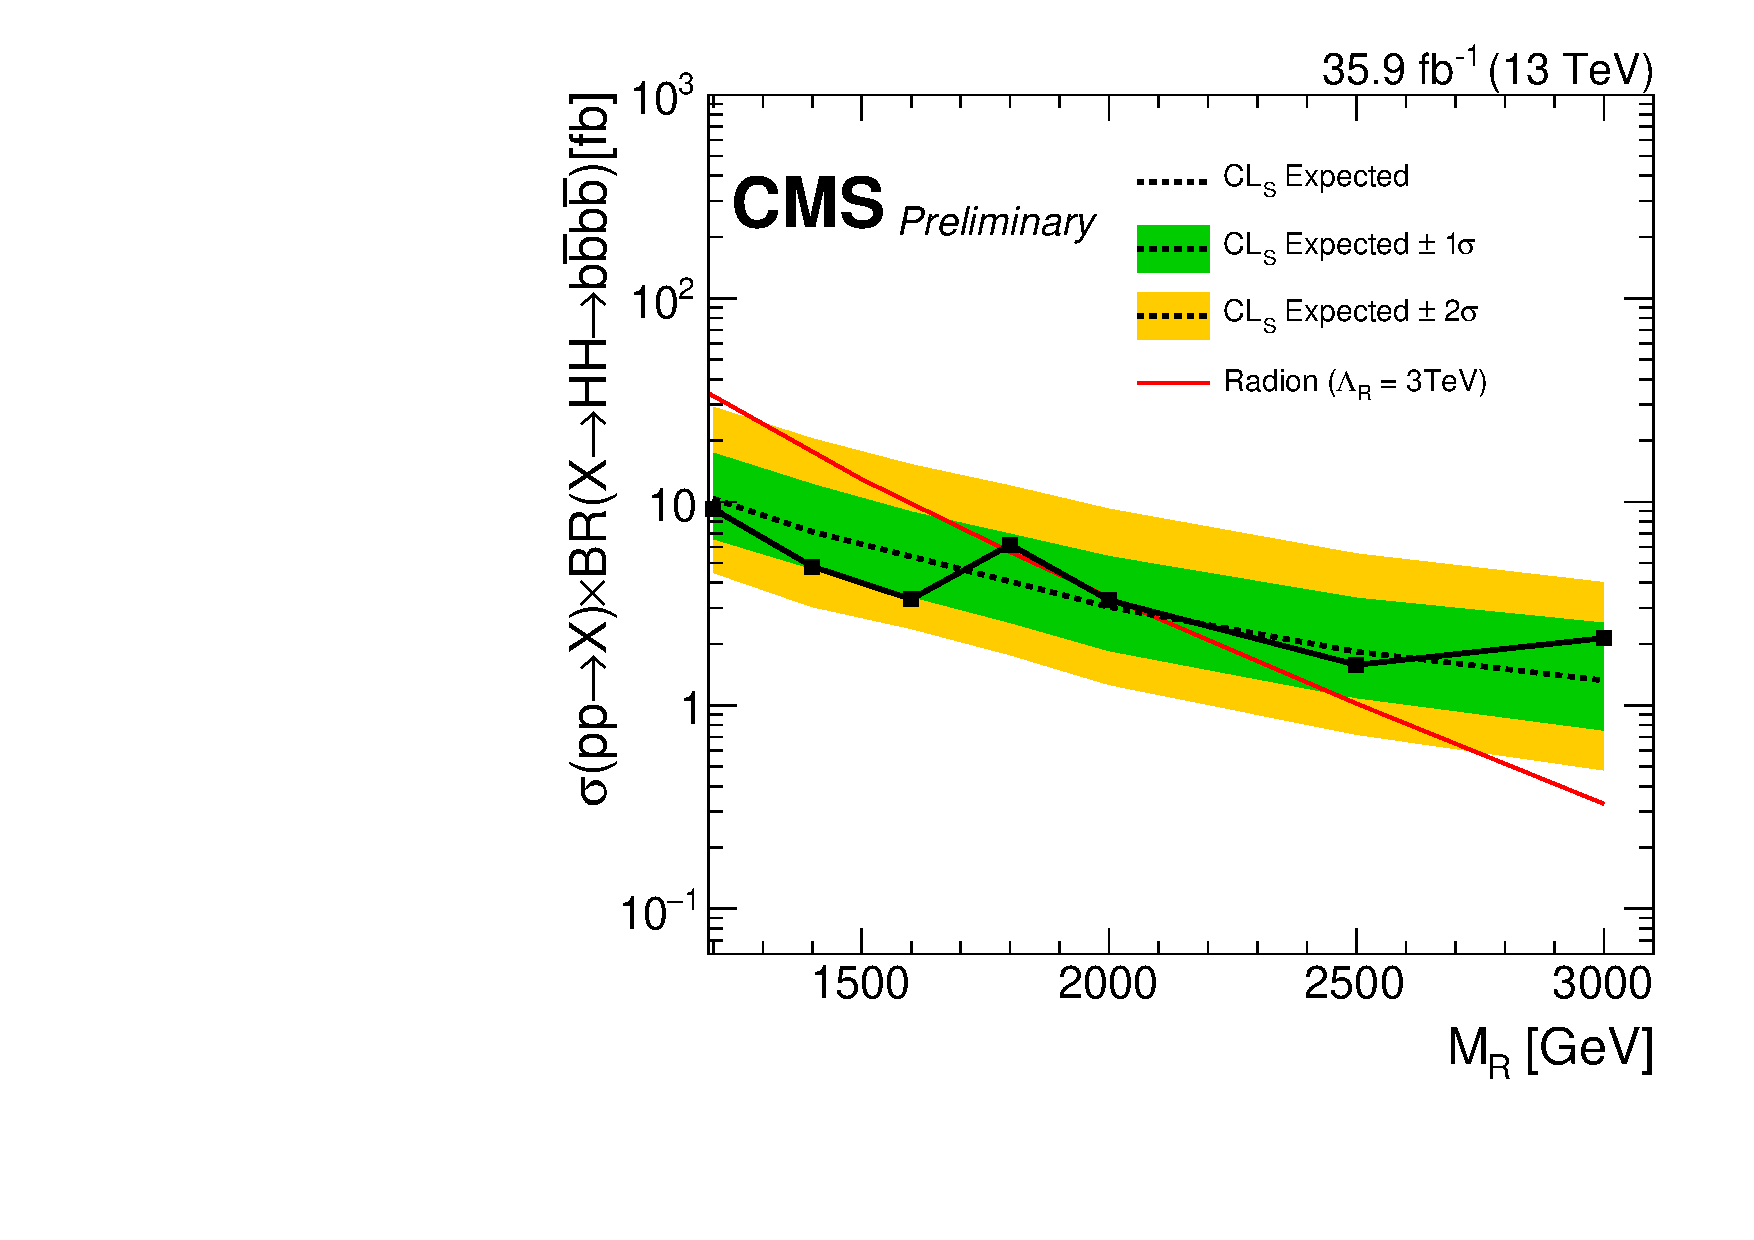
\includegraphics[width=0.5\textwidth]{Figures/central_CW_rd/limit.pdf} \\
  \end{tabular}
  \caption{The 95$\% $ upper limit on signal cross section $\times $ branch ratio (pp $\rightarrow$ X $\rightarrow$ HH $\rightarrow b\bar{b}b\bar{b}$) of bulk graviton (left) and radion (right).}
  \label{fig:hvt_brs}
\end{figure} 

\begin{table}[]
\centering
\label{my-label}
\begin{tabular}{|l|l|l|l|l|}
\hline
\multicolumn{1}{|c|}{\multirow{2}{*}{Mass Point (GeV)}} & \multicolumn{4}{c|}{Upper Limit (fb)}                                                                                                                                                                                                                        \\ \cline{2-5} 
\multicolumn{1}{|c|}{}                                  & \begin{tabular}[c]{@{}l@{}}Radion\\ Expected\end{tabular} & \begin{tabular}[c]{@{}l@{}}Radion\\ Observed\end{tabular} & \begin{tabular}[c]{@{}l@{}}Bulk Graviton\\ Expected\end{tabular} & \begin{tabular}[c]{@{}l@{}}Bulk Graviton \\ Observed\end{tabular} \\ \hline
1200                                                    & 10.0                                                      & 9.2                                                       & 6.9                                                              & 6.3                                                               \\ \hline
1400                                                    & 7.1                                                       & 4.8                                                       & 5.0                                                              & 3.5                                                               \\ \hline
1600                                                    & 5.4                                                       & 3.3                                                       & 3.6                                                              & 2.3                                                               \\ \hline
1800                                                    & 4.1                                                       & 6.2                                                       & 2.6                                                              & 3.9                                                               \\ \hline
2000                                                    & 3.0                                                       & 3.3                                                       & 2.1                                                              & 2.4                                                               \\ \hline
2500                                                    & 1.8                                                       & 1.6                                                       & 1.2                                                              & 1.1                                                               \\ \hline
3000                                                    & 1.3                                                       & 2.1                                                       & 0.9                                                              & 1.5                                                               \\ \hline
\end{tabular}
\caption{The table of 95$\% $ upper limit on signal cross section $\times $ branch ratio (pp $\rightarrow$ X $\rightarrow$ HH $\rightarrow b\bar{b}b\bar{b}$).}
\end{table}

\section{Conclusion}
Searches for heavy resonances above 1.2 TeV decaying to a pair of Higgs
bosons in the four b quark final state using 35.9$fb^{-1}$ proton-proton collison data at center-of-mass energy 13 TeV collected with the CMS detector at the LHC are presented. The background is exstimated by alphabet assisted bump hunt. The systematic uncertainties are mainly from double-b tagger scale factor, Higgs tagging, and $\tau_{21}$ scale factor. Bulk graviton and Radion are considered as signal. There is no excess from expected background in data. The 95 $\% $ confident level CLs of upper limit on cross section $\times$ branch ration (pp $\rightarrow$ X $\rightarrow$ HH $\rightarrow b\bar{b}b\bar{b}$) of both signal are below 10 fb above 1.2 TeV. Bulk graviton is not excluded in the mass region from 1.2 TeV to 3 TeV, while radion is excluded from 1200 GeV to 1787 GeV and from 1964 GeV to 2078 GeV. 
 